\begin{figure}[ht]
    \centering
    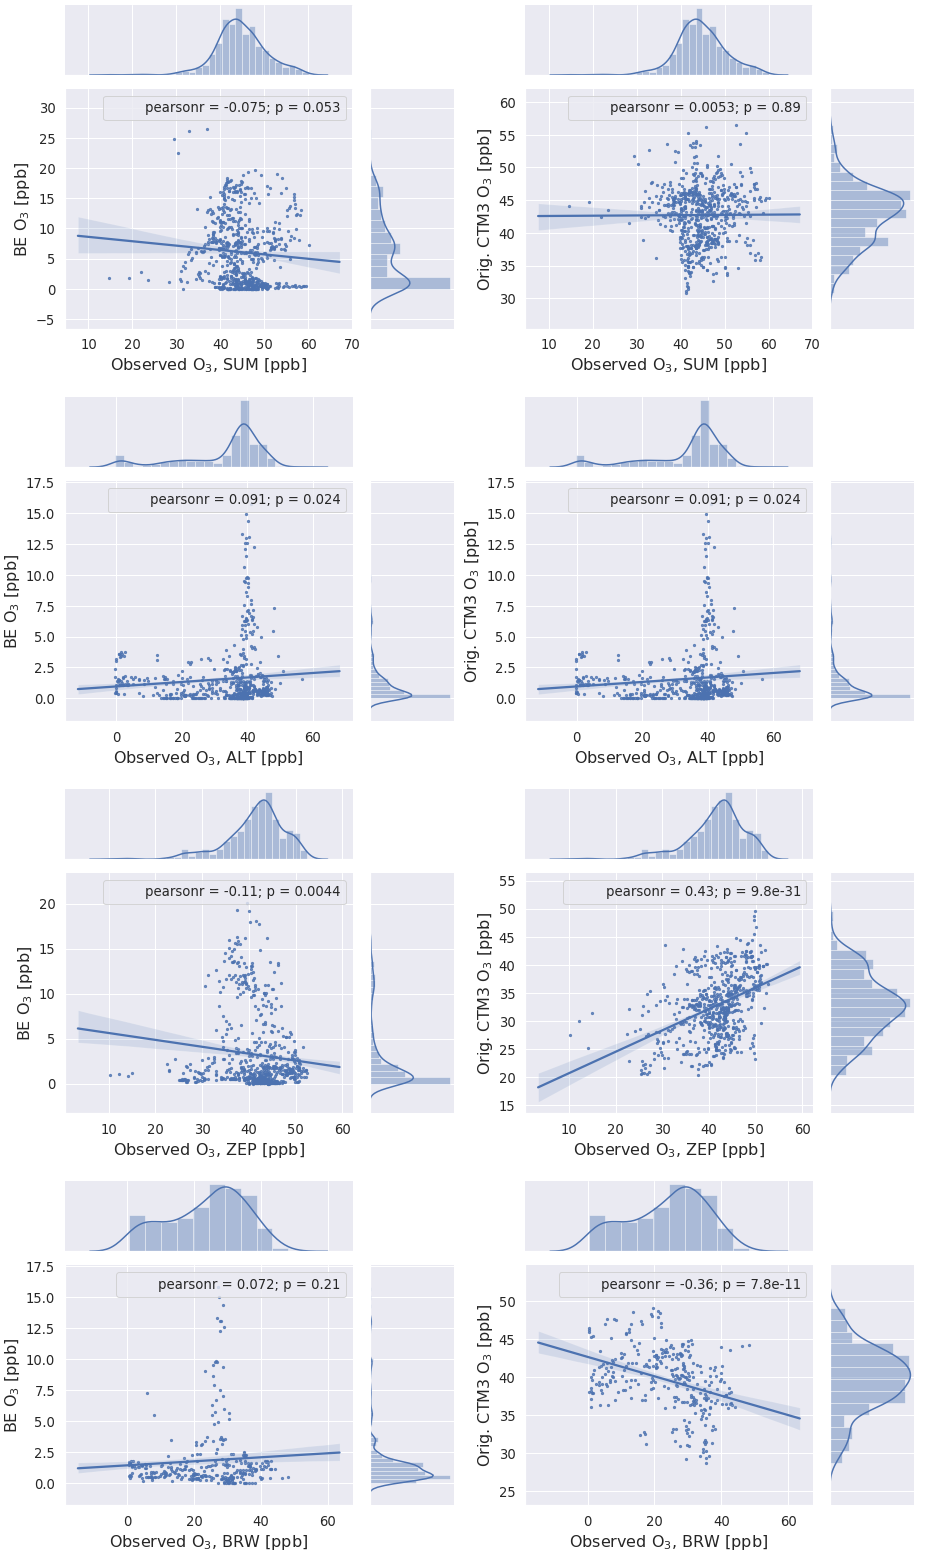
\includegraphics[width = 0.8\linewidth]{Chapter6_Results/images/Orig_BE_comp/jointplot_FebApr_O3_2001.png}
    \caption{Measured $\chem{O_3}$ in ppb vs. modelled results from the and modelled results from the BE-branch (left columns) and original CTM3 (right columns) at the four stations, Summit (SUM), Alert (ALT), Barrow(BRW) and Zeppelin(ZEP) (model results taken from the station's approximate altitude). The histogram distribution of the observations (x-axis) and the model results (y-axis) are shown on the x- and y-axis, respectively. The Pearson correlation coefficient and p-value is shown in the top right corner. \textbf{Period 1} - February 1st-April 24th, 2001}
    \label{fig:joint_FebApr}
\end{figure}


